\documentclass[11pt]{beamer}

\usetheme{Warsaw}
\usepackage{mathrsfs}
\usepackage{amsmath}
\usepackage{graphicx}
\usepackage{caption}
%\usepackage{subcaption}

%Mathematical writting
\theoremstyle{plain}
\newtheorem{thm}{Theorem}[section]

\theoremstyle{definition}
\newtheorem{dfn}{}[section]

%New commands
\newcommand\ChangeFont{\fontsize{9}{7.2}\selectfont}
\newcommand{\y}{\textbf{y}}
\newcommand{\x}{\textbf{x}}

\newcommand{\p}{\mathbb{P}}
\newcommand{\like}{\p_{like}}
\newcommand{\prior}{\p_{prior}}
\newcommand{\post}{\p_{post}}

\begin{document}
%Presentation slide

\begin{frame}{Thesis Defence}
\begin{center}
\large{Simon Fraser University}
\end{center}
\begin{figure}

\includegraphics[scale=0.15]{log}
\end{figure}
\begin{center}
Parameter Estimation Using Gaussian Process Regression.
\end{center}

\begin{center}
Juan Gabriel Garc{\'i}a
\end{center}

\begin{center}
April 10 of 2018
\end{center}
\end{frame}

\AtBeginSection[] 
{ 
\begin{frame} 
\ChangeFont 
\frametitle{Content} 
\tableofcontents[currentsection] 
\end{frame} 
} 











\section{Overview}
\begin{frame}{Problem of Interest}

Given a function
\begin{equation*}
u:A\times\Theta\rightarrow \mathbb{R},
\end{equation*}
where $A\subset\mathbb{R}^{n}$ and $\Theta$ is a set of parameters. Given
experimental (noisy) measures of $u$ at known points $\textbf{x}_{1},\ldots,\textbf{x}_{n}\in A$.
How to infer the values of the parameters in $\Theta$ and their uncertainties when 
$u$ is computationally expensive?

\end{frame}

\begin{frame}{Case Study}

\begin{columns}[c]
\column{1.5in}
Consider the model of pollutant transport for the concentration $c$ of a pollutant
\begin{equation*}
\partial_{t} c+L(\theta)c=f
\end{equation*}
Goal: Estimate $Q_{i}$ and $\theta$ using measurements of deposition in  $R_{j}$.
\column{1.5in}
\begin{figure}
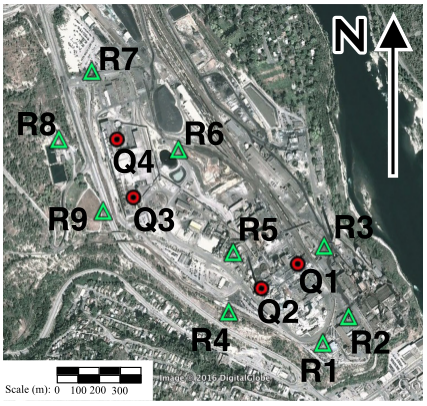
\includegraphics[scale=0.36]{BCtrail}
\ChangeFont
\end{figure}

\end{columns}
\end{frame}




\begin{frame}{Case Study}
\begin{equation*}
\partial_{t} c(\textbf{x},t)+\nabla\cdot(\textbf{u}(\textbf{x},t)c+\textbf{S}(\textbf{x},t)\nabla c)
=q(\textbf{x},t)\qquad\text{on }\mathbb{R}^{2}\times\mathbb{R}_{\geq 0}\times(0,T).
\end{equation*}
\begin{itemize}
\item $\textbf{u}(\textbf{x},t)=(u_{x}(z,t),u_{y}(z,t),u_{set})$ 
(Wind velocity field)
\item $\|(u_{x},u_{y})\|_{2}\propto\left(\frac{z}{z_{r}}\right)^{\gamma}$.
\item $\textbf{S}=diag(s_{x},s_{y},s_{z})$ (Eddy diffusion matrix)
\item $s_{z}=f(L,z_{cut})$, where $\frac{1}{L}=a+b\log_{10}(z_{0})$.
\item $s_{x}=s_{y}=g(z_{i},L)$, with $z_{i}$ Mixing layer height.
\end{itemize}
\end{frame}



\begin{frame}{Case Study}
In this slide expand a little on the model,
like initial conditions and such
\end{frame}


\begin{frame}{Steps}
How to proceed?
\begin{enumerate}
\item Find a surrogate for $u$.
\item Locate the optimal points to evaluate $u$ so that the surrogate is accurate.
\item See if it is possible to do dimensionality reduction
\item Use the Bayesian framework to obtain the posterior distribution of the parameters 
in the light of the experimental data
\item Perform inference on the posterior using numerical methods.
\end{enumerate}
\end{frame}  


\section{Finding a Surrogate for $u$}


\begin{frame}{Gaussian Process}
\begin{dfn} 
A Gaussian process (GP) is a collection of random variables $\{g(x)\}_{x\in A}$, for some set $A$,
possibly uncountable,
 such that any finite subset of random variables
 $\{g(x_{k})\}_{k=1}^{N}\subset\{g(x)\}_{x\in A}$ for
$\{x_{k}\}_{k=1}^{N}\subset A$ are jointly Gaussian.
\end{dfn}
\end{frame}
\begin{frame}
\frametitle{Multivariate Gaussian Distribution}
\begin{dfn}
Two random vectors $X\in\mathbb{R}^{n}$ and $Y\in\mathbb{R}^{m}$
are jointly Gaussian if their joint density function is given by
\begin{equation*}
\frac{1}{(2\pi)^{\frac{m+n}{2}}|\Sigma|^{\frac{1}{2}}}
\exp(-([x,y]-[\mu_{x},\mu_{y}])
\underbrace{\begin{bmatrix}
\Sigma_{xx} & \Sigma_{xy}\\
\Sigma_{xy}^{T} & \Sigma_{yy}
\end{bmatrix}}_{\Sigma}
([x,y]-\underbrace{[\mu_{x},\mu_{y}]}_{\mu})^{T})
\end{equation*}
%In this case we write
%\begin{equation*}
%(X,Y)\sim\mathcal{N}(\mu,\Sigma)
%\end{equation*}
\end{dfn}
\begin{itemize}
\item Marginal distribution is multivariate Gaussian.
	\begin{itemize}
		\item $X\sim\mathcal{N}(\mu_{x},\Sigma_{xx})$.
		\item $Y\sim\mathcal{N}(\mu_{y},\Sigma_{yy})$.
	\end{itemize}
\item Conditional distribution is multivariate Gaussian.
	\begin{itemize}
		\item $X|Y=y\sim\mathcal{N}(\mu_{x}-\Sigma_{xy}\Sigma_{yy}^{-1}
		(y-\mu_{y}),\Sigma_{xx}-\Sigma_{xy}\Sigma_{yy}^{-1}\Sigma_{yx})$.
	\end{itemize}
\end{itemize}
\end{frame}

%In this section you introduce everything that is related to GPs

\begin{frame}
\frametitle{Gaussian Process as Interpolator}
\begin{figure}
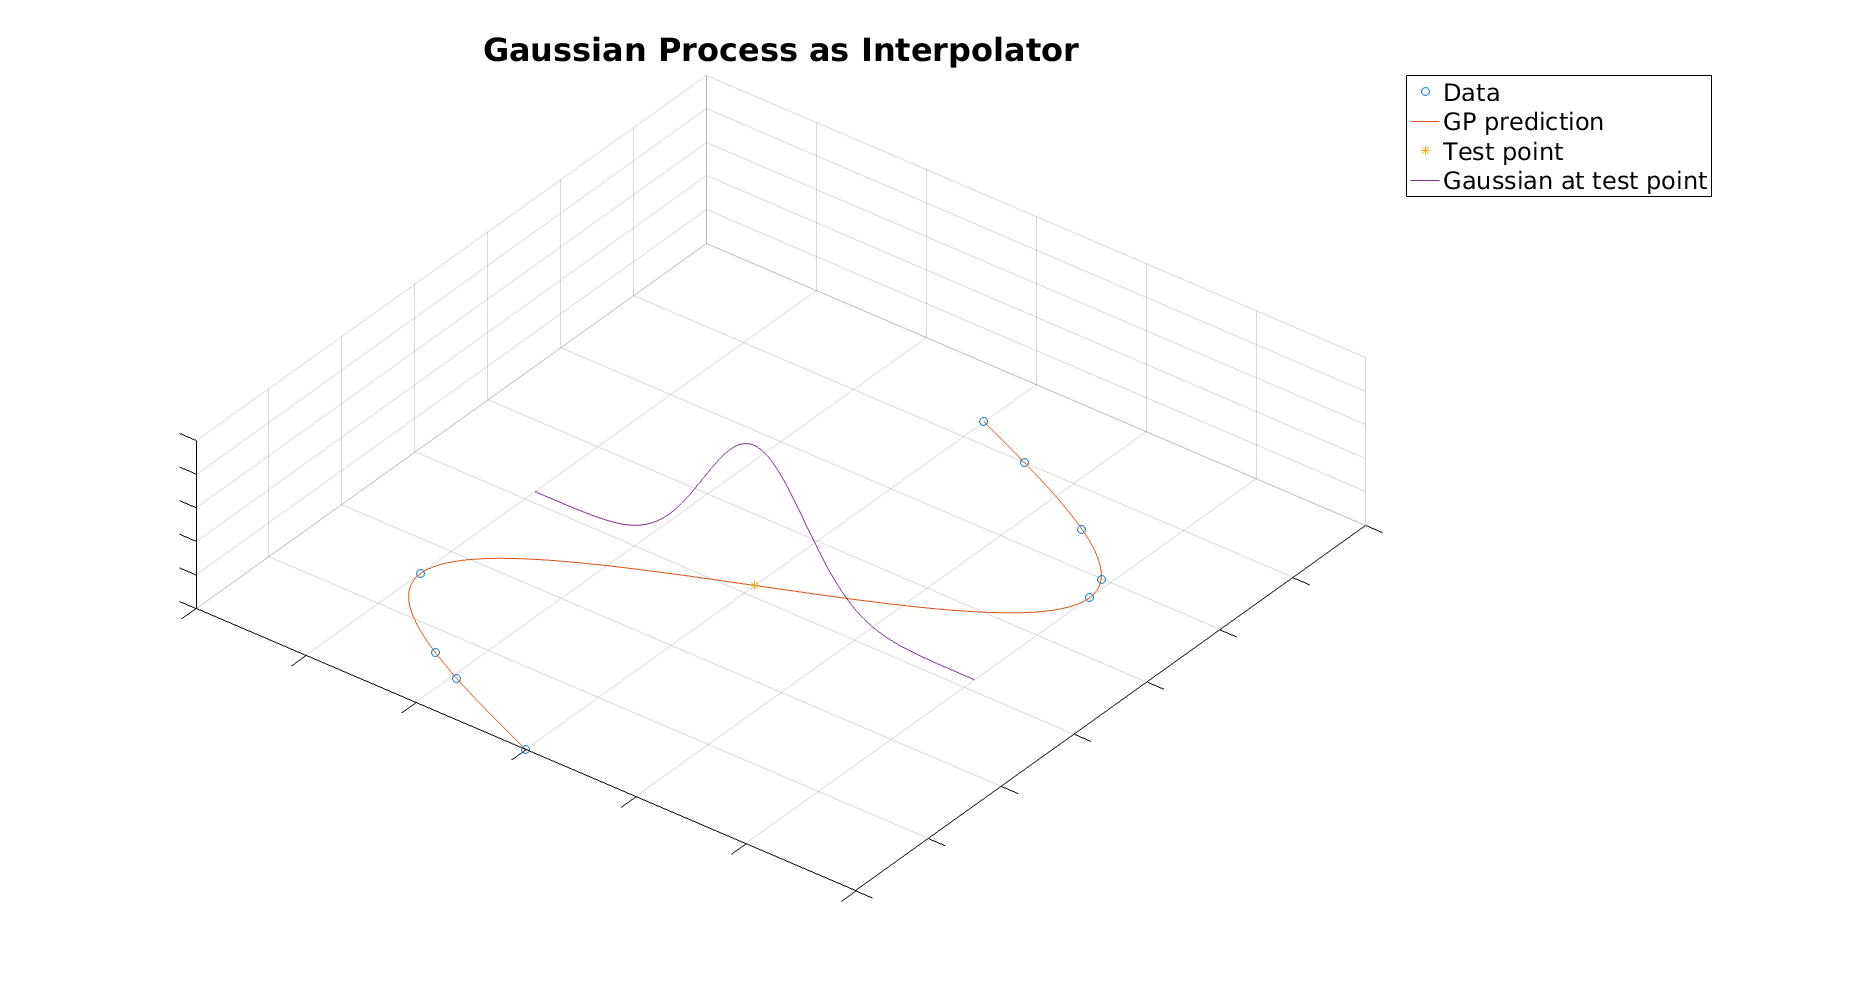
\includegraphics[scale=0.25]{./codes/Gp_interpolation.png}
\end{figure}

\end{frame}


\begin{frame}
\begin{figure}
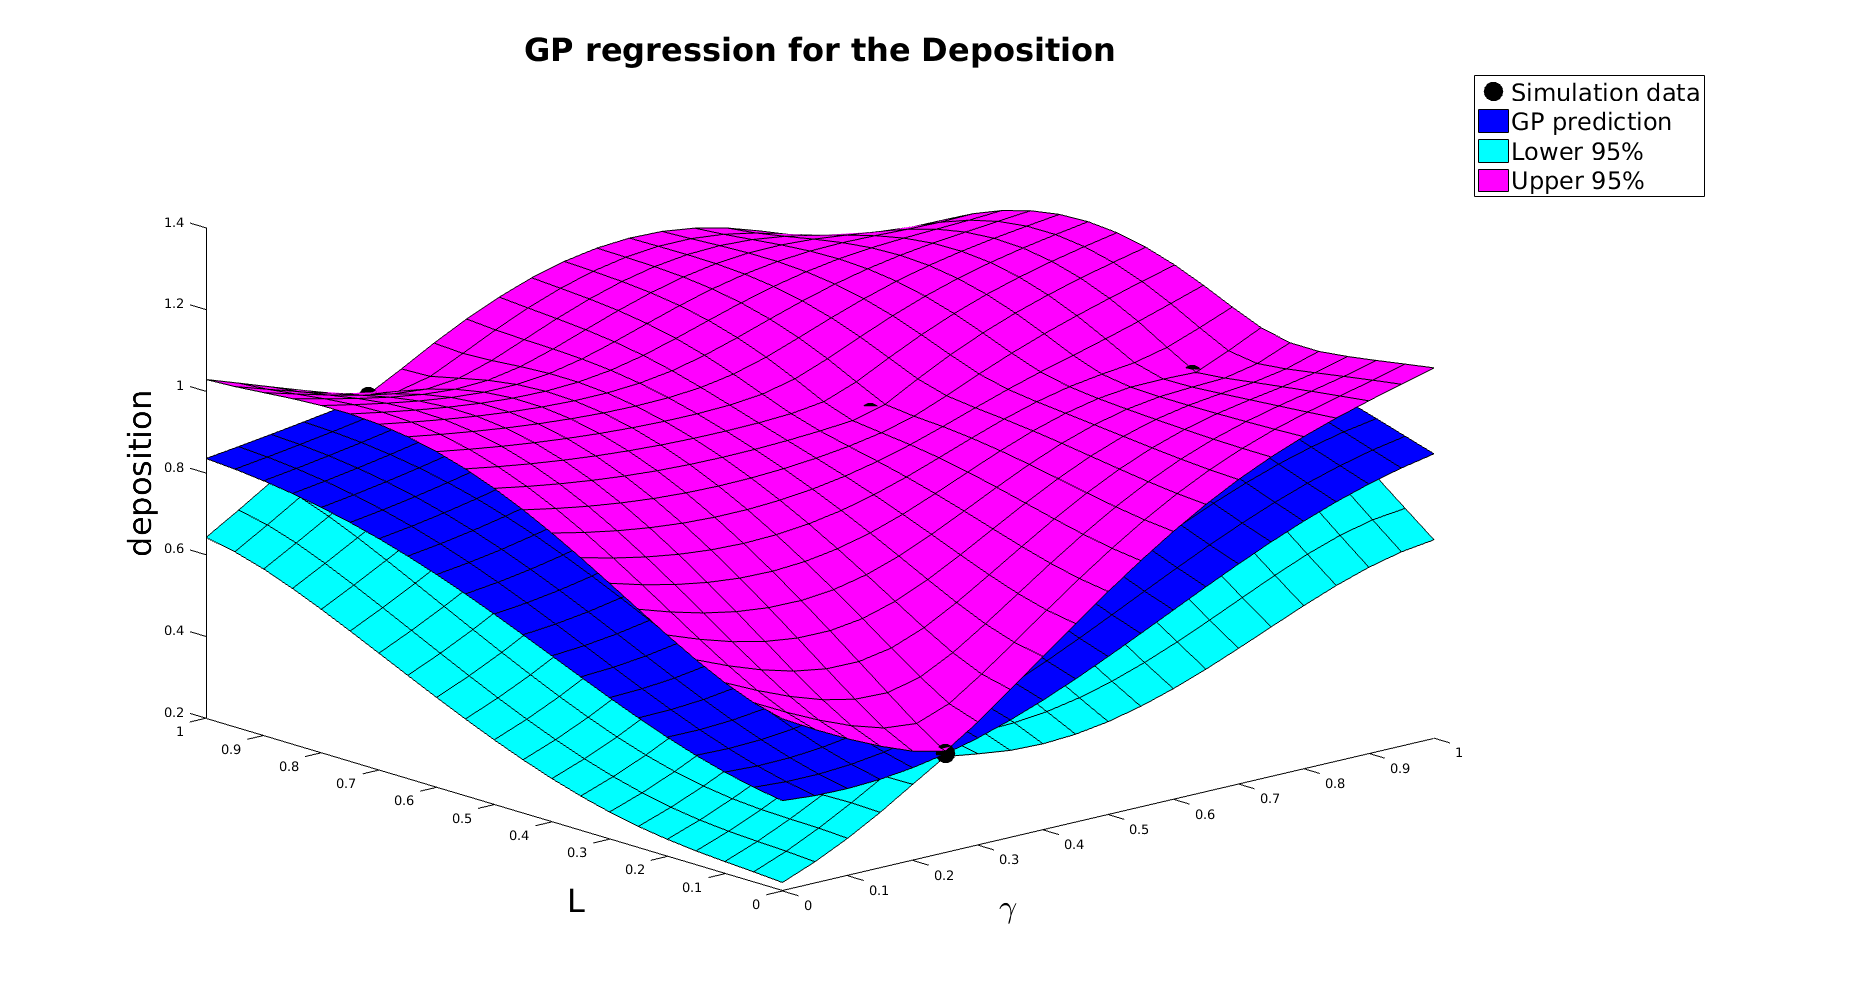
\includegraphics[scale=0.2]{./codes/GP_regression.png}
\end{figure}
\end{frame}
\section{Optimizing the Surrogate interpolation Capabilities}


\begin{frame}{Why Experimental Design}
\begin{figure}
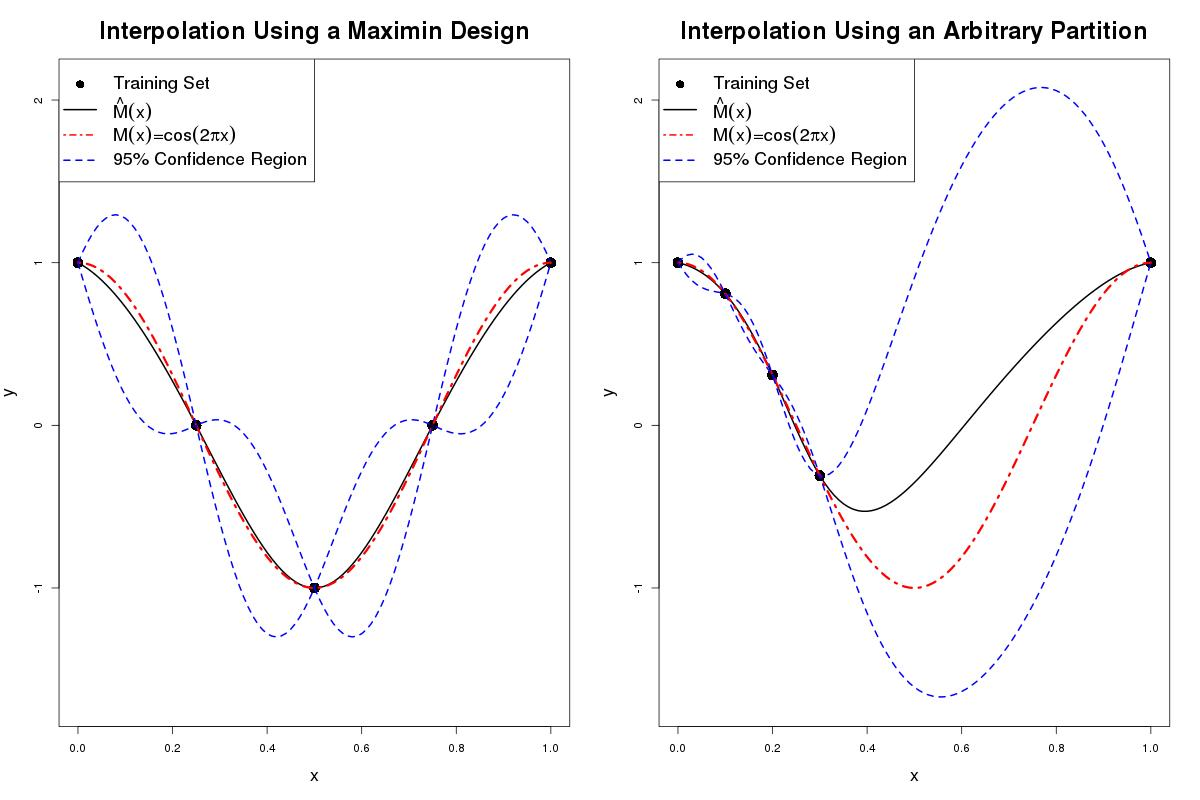
\includegraphics[scale=0.2]{../FigChap2/partitionComparison.jpg}
\end{figure}

\end{frame}

\begin{frame}{Maximin Design}
In this slide you talk about maximin design
\end{frame}

\begin{frame}{Example of a design}
\begin{figure}
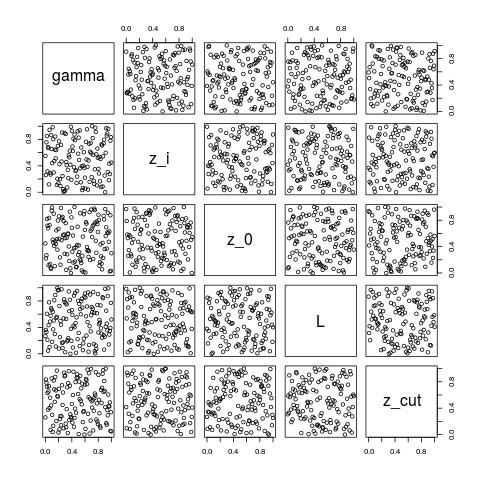
\includegraphics[scale=0.35]{./codes/experimental_design128.png}
\end{figure}

\end{frame}
%Here comes the part when you talk about design of experiments

\section{Reducing the Complexity of the Model}

\begin{frame}{Sobol Indices}
\ChangeFont
To assess the relevance of the parameters we do a Sensitivity analysis.
\begin{itemize}
\item Given a function of interest $\varphi$ we decompose it as 
\begin{equation*}
\varphi(x_{1},\ldots,x_{n})=\varphi_{0}+\sum_{k=1}^{n}\varphi_{k}(x_{k})+
\sum_{1\leq k< l\leq n}\varphi_{kl}(x_{k},x_{l})+\ldots+
\varphi_{1,2,\ldots,n}(x_{1},\ldots,x_{n}).
\end{equation*}
\item With the constraint
\begin{equation}\label{eqnSobolCond1}
\int_{[0,1]}\varphi_{i_{1},\ldots,i_{j}}dx_{i_{k}}=0\qquad\text{if }  i_{k}\in \{i_{1},\ldots,i_{j}\}
\end{equation}
\item This condition allows to find each element in the decomposition recursively.
\end{itemize}
\end{frame}

\begin{frame}
\frametitle{Sobol Indices}
The total variance $D$ of $\varphi$ is defined as
\ChangeFont
\begin{equation*}
D=\int_{\Omega^{n}}\varphi^{2}(x)dx-\varphi_{0}^{2}.
\end{equation*}
Similarly we can compute the partial variances as
\begin{equation*}
D_{i_{1},\ldots,i_{s}}=\int_{[0,1]^{n-1}}\varphi^{2}_{i_{1},\ldots,i_{s}}dx_{i_{1}}\ldots dx_{i_{s}}.
\end{equation*}
With these variances we define the $s-th$ order  Sobol index
\begin{equation*} 
S_{i_{1},\ldots,i_{s}}=\frac{D_{i_{1},\ldots,i_{s}}}{D}.
\end{equation*}
To measure the relevance of the $i$-th parameter we calculate
\begin{equation*}
S_{i}+S_{i1}+S_{i2}+\ldots+S_{i12}+S_{i13}+\ldots+S_{12\ldots,i,\ldots, n}.
\text{ (Total Sobol Index)}
\end{equation*}
\end{frame}


\begin{frame}
\frametitle{Sensitivity Analysis}
\begin{columns}[c]
\column{1.5in}
\ChangeFont
\begin{itemize}
\item $\gamma$: Fitting parameter for the z dependence of the velocity.
\item $z_{0}$: Roughness length.
\item $z_{i}$: Mixing layer height.
\item $L$: Monin-Obukhov length.
\item $z_{cut}$: cutoff height.
\end{itemize}

\column{1.5in}
\begin{figure}
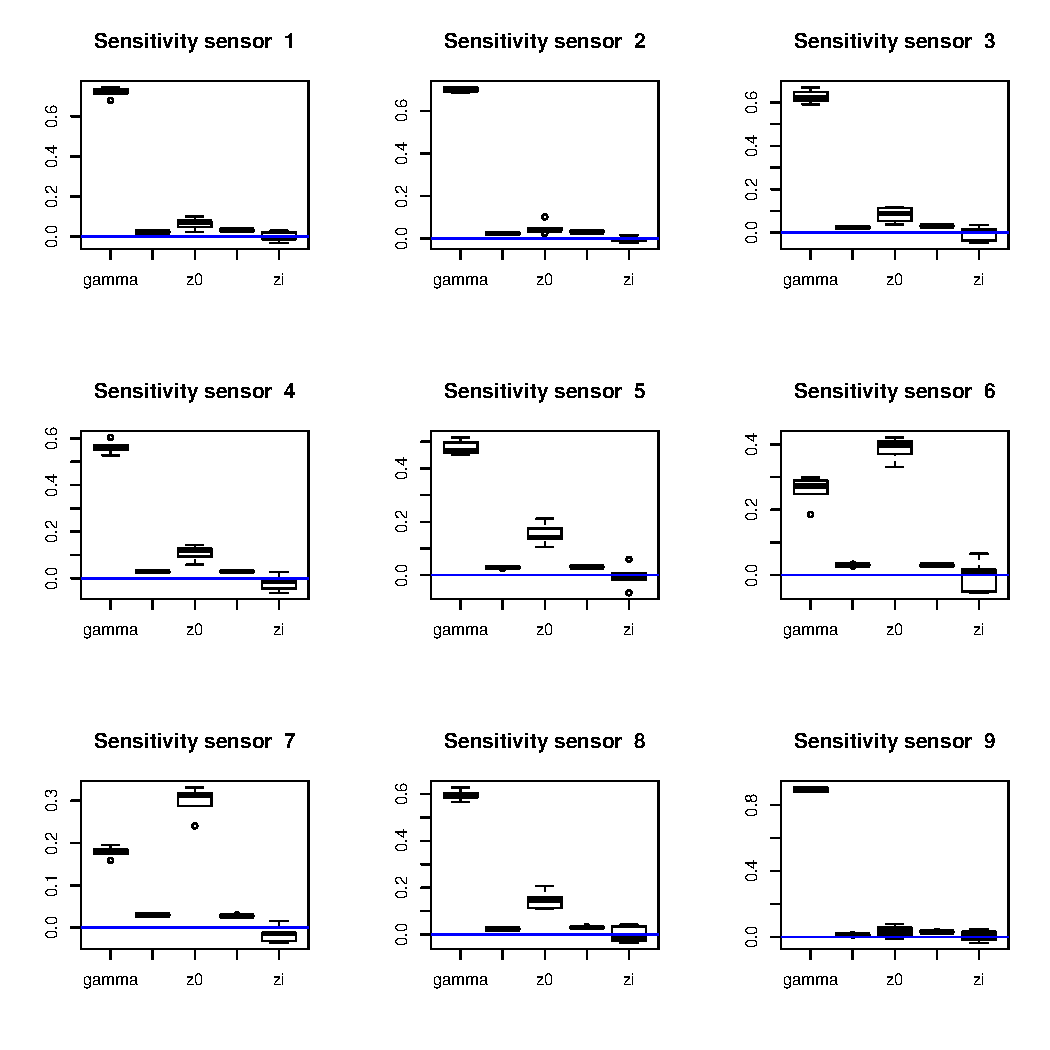
\includegraphics[scale=0.3]{../FigChap4/sensitivityPlot.pdf}
\end{figure}

\end{columns}
\end{frame}

\begin{frame}
In this frame it is necessary to explain why you add an $\epsilon$ for the noise and stuff

\end{frame}


\begin{frame}
\frametitle{What About the Sources?}

\begin{dfn}
The deposition behaves linearly  with respect to the values of the 4  sources,
hence
\begin{equation*}
\begin{bmatrix}
R_{1} \\
R_{2} \\
\vdots\\
R_{9}
\end{bmatrix}=A(\gamma,z_{0},L)
\begin{bmatrix}
q_{1}\\
\vdots\\
q_{4}
\end{bmatrix}
+\vec{\epsilon},\qquad\text{ where } \vec{\epsilon}\sim\mathcal{N}(0,
\sigma^{2}I_{9\times 9}).
\end{equation*}
To evaluate the matrix $A(\gamma,z_{0},L)$ in points $(\gamma,z_{0},L)$ outside the experimental design we fit a 
Gaussian process in each of the 36 entries of $A(\gamma,z_{0},L)$.
\end{dfn}
\end{frame}

\begin{frame}
In this frame explain how, now everything is a
random variable and proceed to introduce the
bayesian model
\end{frame}


\section{Introducing the Bayesian Framework}


\begin{frame}
\frametitle{Probabilistic Model}

\begin{dfn}
Our goal is to estimate the values of $p:=(\gamma,z_{0},L)$ and 
$q:=(q_{1},q_{2},q_{3},q_{4})$ given the measurements
$\vec{R}$. Mathematically we want to estimate:

\begin{equation*}
\post(p,q|\vec{R})\propto
\underbrace{\like(\vec{R}|p,q)\prior(p)\prior(q)}_{\text{Assuming $p$ and $q$ independent}}
\end{equation*}
We assume $p\sim Uniform$ over the domain of definition of the parameters.
 
\end{dfn}
\end{frame}

\begin{frame}
\frametitle{What about $q$?}
To set a prior for $q$ we first need to check what do we know about $q$. This knowledge can be 
summarized as follows
\begin{itemize}
\item $q_{k}>0$ for $k=1,2,3,4$.
\item If we trust the engineers the most likely value for $q$ is the engineers estimate.
\item If we think they know what they are doing the true value for $q$ cannot be very far away from their
estimate.
\end{itemize}
\end{frame}

\begin{frame}
\frametitle{Choosing a prior for $q$}
\begin{columns}[c]
\column{2.2in}
A consistent assumption is $q_{k}\sim Ga(\alpha_{k},\beta_{k})$,for $k=1,2,3,4$,
the following conditions that define $\alpha_{k}$ and $\beta_{k}$ for all $k$ uniquely.

\begin{itemize}
\item $\beta_{k}(\alpha_{k}-1)=q_{eng,k}$
\item $qgamma(0.99,\alpha_{k},\beta_{k})=3q_{eng,k}$
\end{itemize}
\column{1.5in}
\begin{figure}
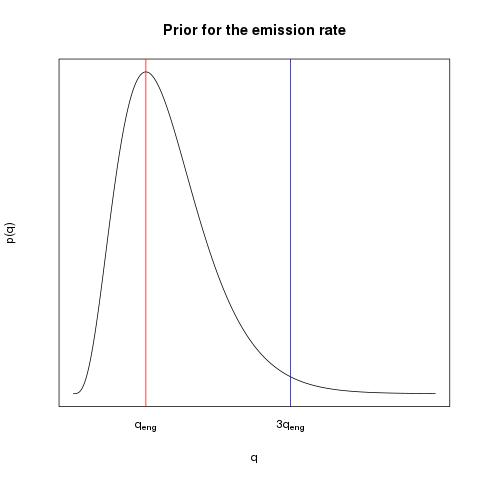
\includegraphics[scale=0.3]{gamma_generic}
\end{figure}
\end{columns}
\end{frame}


\begin{frame}
\frametitle{Getting the posterior}
\begin{itemize}
\item We have $\like(\vec{m}|q,p)\propto
\exp(-\frac{1}{2\sigma_{\epsilon}^{2}}\|m-A(p)q\|^{2}_{2})$
\item Also $\prior(q_{k})\propto q_{k}^{\alpha_{k}-1}\exp(\beta_{k}q_{k})$.
\item and $\prior(p)\propto\textbf{1}_{[0.1,0.4]\times[10^{-3},2]\times[-500,-1]}
:=\textbf{1}_{B}$
\end{itemize}
\bigskip
Then
\newline 
\newline
$\post(q,p|\vec{m})\propto
\textbf{1}_{B}\left(\prod_{k=1}^{4}q_{k}\right)\exp(-\frac{1}{2\sigma_{\epsilon}^{2}}\|\vec{m}-A(p)q\|^{2}_{2}+
\sum_{k=1}^{4}\beta_{k}q_{k})$.
\end{frame}




\section{Decoding the Posterior}
\begin{frame}
In a couple of frames, talk about MCMC methods
\end{frame}

\begin{frame}
Finally show the results you got
\end{frame}
%Finally explain the MCMC techniques









\end{document}
